\chapter{Generador de Chirp}
\section*{Resumen}
El generador de chirp constituye el núcleo fundamental de un radar de onda continua de frecuencia modulada (FMCW). Su propósito principal es sintetizar una señal de microondas cuya frecuencia varíe linealmente con el tiempo, garantizando linealidad, estabilidad, repetitividad y un ancho de banda definido \cite{Andy Harrison}.

\section{Fundamentos de la Modulación de Frecuencia Lineal (LFM)}
En los sistemas de radar FMCW, la capacidad para determinar la distancia y la velocidad de un objetivo depende de la modulación de la señal transmitida \cite{Andy Harrison}. 

Una señal \textit{chirp} se caracteriza por tener una frecuencia instantánea que varía linealmente con respecto al tiempo. Matemáticamente, la frecuencia instantánea $f(t)$ de un \textit{chirp} ascendente (\textit{up-chirp}) se expresa en la Ecuación~\ref{eq:eq3.1}:
\begin{equation}
    f(t) = f_0 + \mu t \quad \text{para} \quad 0 \leq t \leq T_c
    \label{eq:eq3.1}
\end{equation}

Donde $f_0$ es la frecuencia inicial, $T_c$ es el tiempo de barrido (o período del \textit{chirp}), y $\mu$ representa la pendiente de la rampa de frecuencia, definida como la relación entre el ancho de banda total del barrido ($B$) y el tiempo de barrido:
\begin{equation}
    \mu = \frac{B}{T_c}
    \label{eq:pendiente_chirp}
\end{equation}

El ancho de banda $B$ es un parámetro crítico, ya que determina directamente la resolución en rango (distancia) del sistema radar. Por otro lado, la linealidad de la rampa es fundamental, dado que cualquier desviación o no linealidad en $\mu$ se traduce en un ensanchamiento del espectro de la señal de batido en el receptor, degradando la precisión de la medición.

La señal en el dominio temporal $s(t)$ se describe mediante la siguiente expresión:
\begin{equation}
    s(t) = A \cos\!\left(2\pi\left(f_0 t + \frac{\mu}{2} t^2\right)\right) \quad \text{para} \quad 0 \leq t \leq T_c
    \label{eq:senal_chirp_tiempo}
\end{equation}

La representación en el tiempo y espectrograma es la siguiente:
\begin{figure}[H]
    \centering
    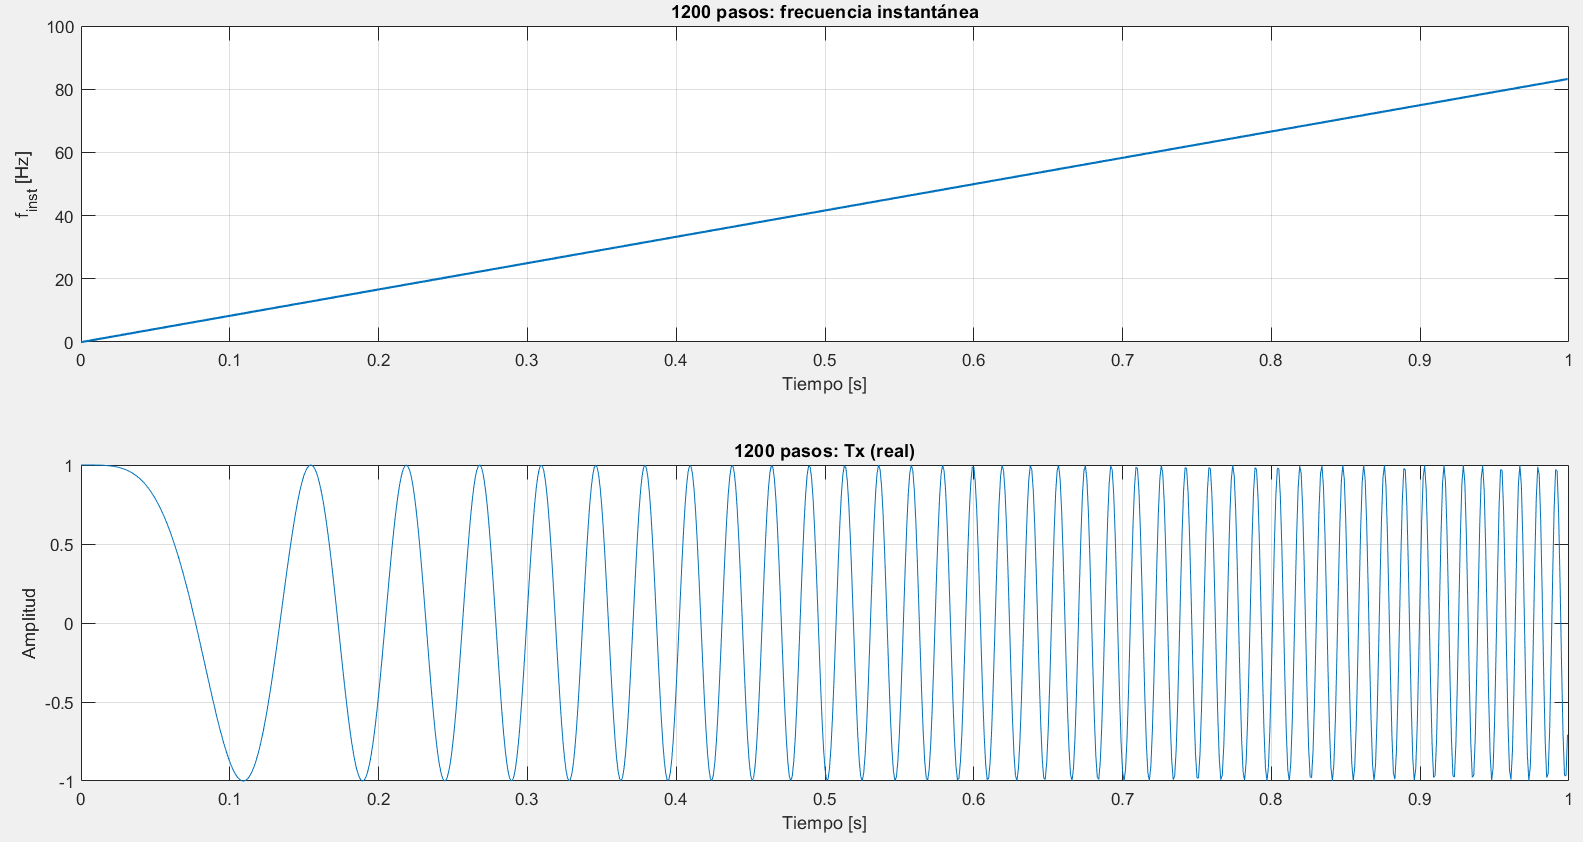
\includegraphics[width=1\linewidth]{imagenes/chirp teorico.png}
    \caption{Señal de la Modulación de Frecuencia Lineal. La imagen superior muestra el chirp diente de sierra a lo largo del tiempo, y la inferior la frecuencia instantánea del chirp diente de sierra, que aumenta linealmente desde 0 hasta $B$ durante el período $T_c$. (Fuente: Generación propia).}
    \label{fig:chirp_diente_sierra}
\end{figure}

\begin{figure}[H]
    \centering
    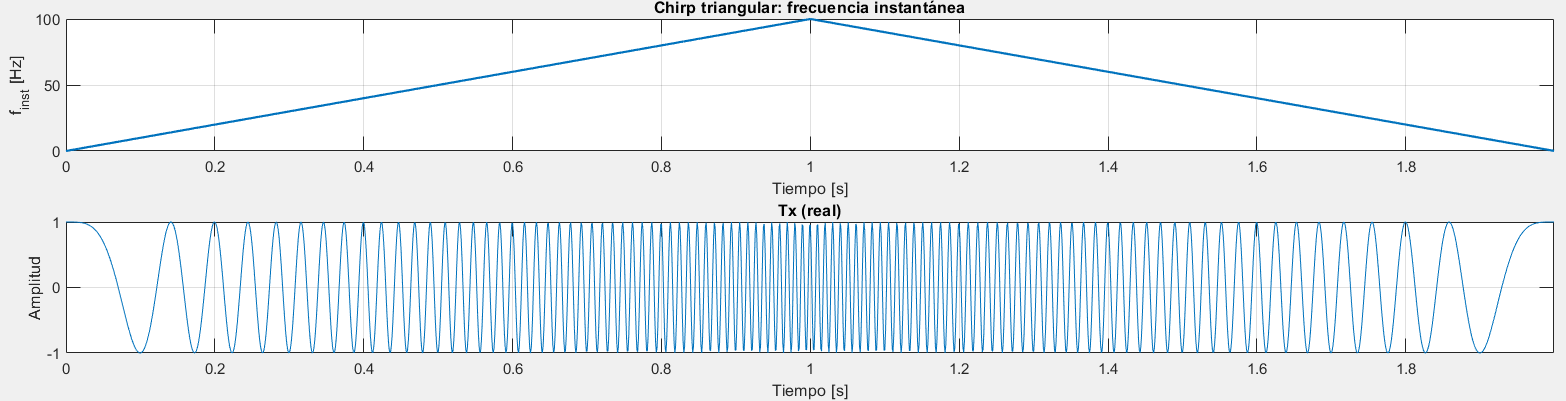
\includegraphics[width=1\linewidth]{imagenes/chirp triangular teorico.png}
    \caption{Señal de la Modulación de Frecuencia Lineal. La imagen superior muestra el chirp triangular a lo largo del tiempo, y la inferior la frecuencia instantánea del chirp triangular, que aumenta linealmente desde 0 hasta $B$ durante el período $T_c$. (Fuente: Generación propia).}
    \label{fig:chirp_triangular}
\end{figure}

La representación de la señal chirp en el dominio de la frecuencia permite visualizar el ancho de banda recorrido durante el barrido. Para un chirp lineal, la frecuencia instantánea varía linealmente entre una frecuencia inicial $f_0$ y una frecuencia final $f_0+B$, donde $B$ representa el ancho de banda del barrido. En consecuencia, el espectro de la señal se encuentra distribuido sobre dicho intervalo de frecuencias.

\begin{figure}[H]
    \centering
    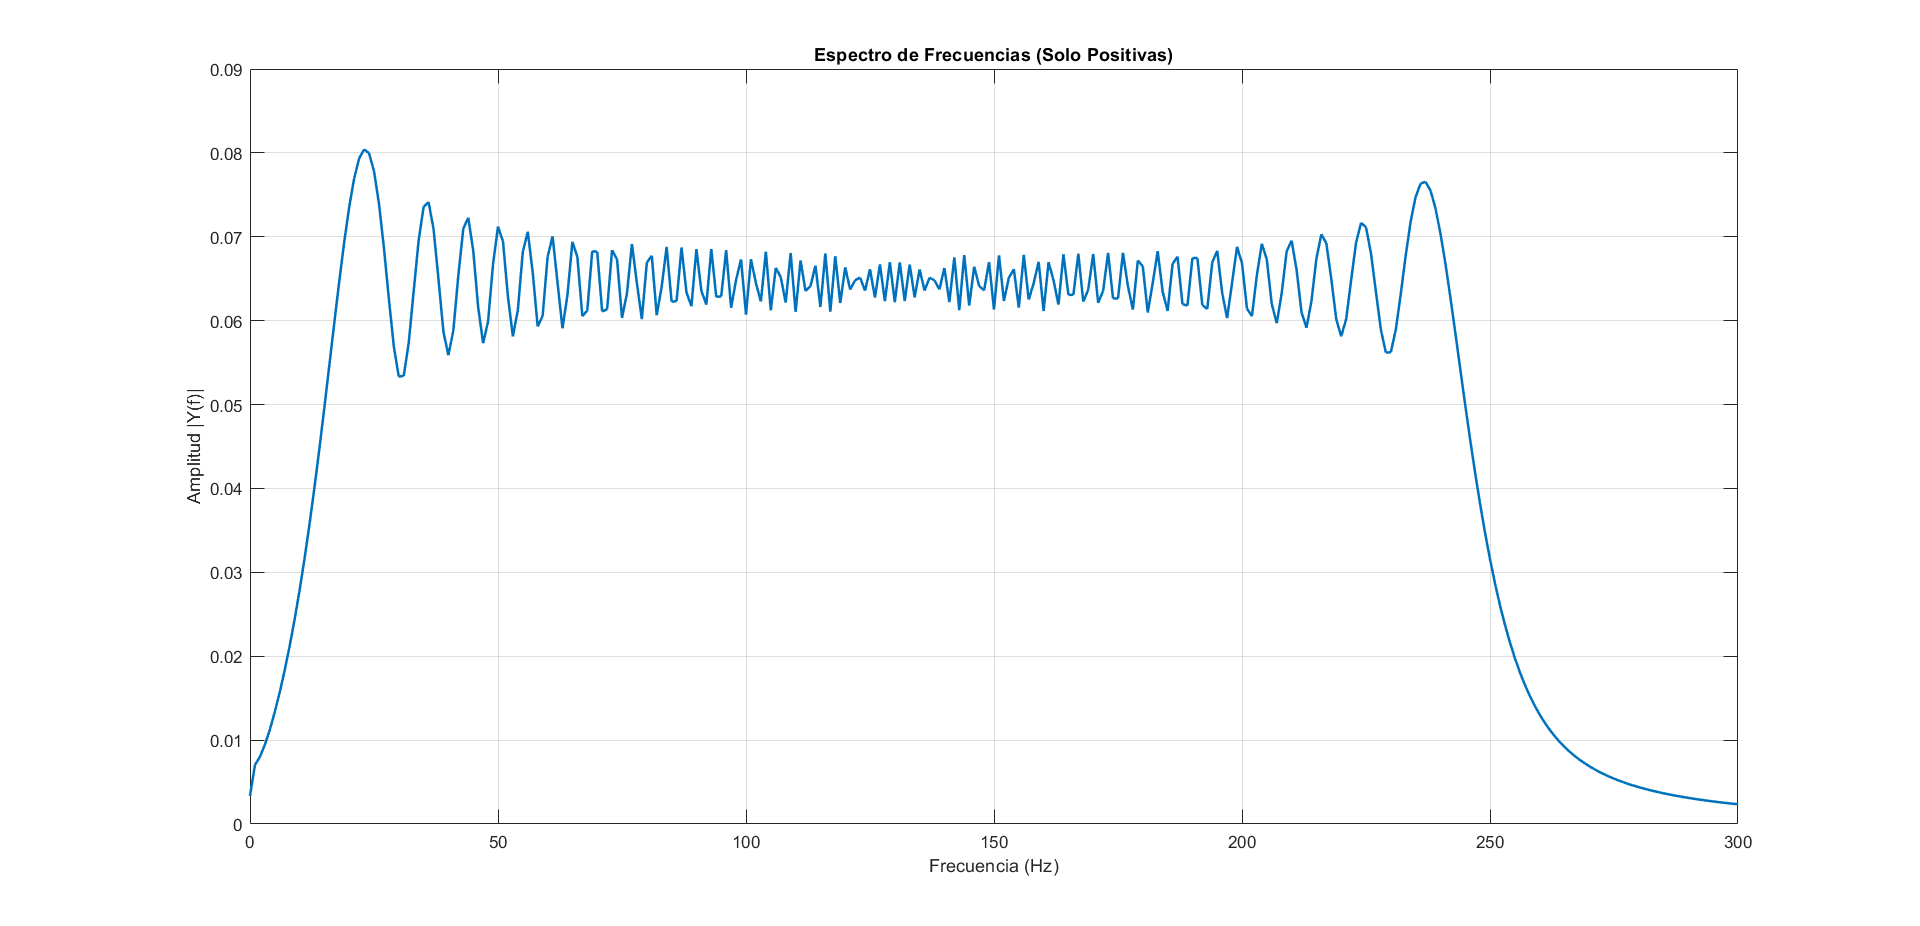
\includegraphics[width=0.85\linewidth]{imagenes/chirp_frecuencia.png}
    \caption{Representación espectral de un chirp lineal. (Fuente: Generación propia).}
    \label{fig:chirp_frecuencia}
\end{figure}